% chapter 3
\chapter{Control Unit}
\label{chap:03_control_unit}

\section{Hardwired Control Unit}
The Control Unit (CU) is responsible for orchestrating the flow of control signals across the pipeline. It takes in the output from Instruction Memory (IRAM), which is determined by the current value of the Program Counter (PC), and contains the instruction to be executed. \\

The architecture of the CU is designed using a hard-wired approach to maximize both reliability and simplicity. Two \textbf{Look-Up Tables} are employed within the combinational logic to generate an \textbf{18-bit Control Word} signal and the \textbf{ALU operational code}. These control signals are then segmented and distributed to the various pipeline stages: fetch, decode, execute, memory and write-back. \\

As previously discussed in Section~\ref{sec:instruction_set}, the instruction set is categorized into three primary types: register-to-register (R-Type), immediate operations (I-Type) and jump instructions (J-Type). The encoding format for each instruction type varies as follows:
\begin{itemize}
    \item \textbf{R-Type}: 6-bit OPCODE, 5-bit operand A (RS1), 5-bit operand B (RS2), 5-bit destination register (RD), and 11-bit FUNC.
    \item \textbf{I-Type}: 6-bit OPCODE, 5-bit operand A (RS1), 5-bit destination register (RD), and 16-bit immediate.
    \item \textbf{J-Type}: 6-bit OPCODE and 26-bit immediate.
\end{itemize}

Upon receiving an instruction, the CU extracts the \textbf{OPCODE} and, in the case of R-type instructions, the \textbf{FUNC} field. The OPCODE informs the CU about the specific type of instruction to be executed, while the FUNC field guides the ALU to perform the corresponding operation. Implicit encoding is chosen for the ALU opcode to improve readability during both the coding and testbench phases. \\

The pipeline accepts a new instruction during each clock cycle, enabling the simultaneous execution of up to five instructions, each at a different stage of the pipeline. To keep the control signals in sync with the pipeline stages, the Control Word and the ALU operational code are shifted by one position with every positive edge of the clock cycle. This ensures that control signals are delivered to the correct pipeline stage in a timely manner, as depicted in Figure~\ref{fig:control_unit}.

\begin{figure}[!htbp]
    \centering
    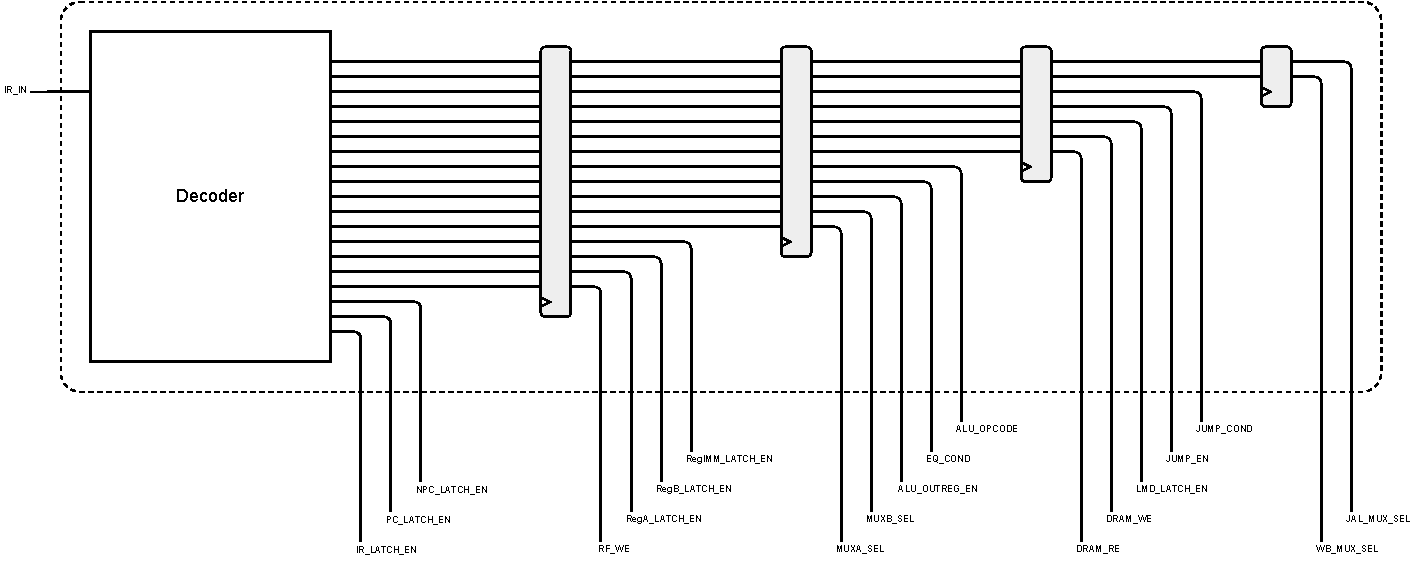
\includegraphics[width=0.98\textwidth]{source/figures/control_unit.pdf}
    \caption{Control Unit}
    \label{fig:control_unit}
\end{figure}

\section{Control Word}
This section describes the control signals produced by the Control Unit to manage the various stages of the DLX pipeline. With the exception of \texttt{ALU\_OPCODE}, that specifies the operation to be performed by the ALU, all other signals are part of the Control Word and are thus 1-bit signals. \\

The signals are presented in reverse order compared to their definitions in the Control Unit module. This is because the Most Significant Bit (MSB) of the Control Word represents the first signal sent to the datapath, specifically \texttt{IR\_LATCH\_EN}. Conversely, position 0 of the Control Word corresponds to the last signal sent to the write-back stage, which is \texttt{JAL\_MUX\_SEL}.

\begin{itemize}%[nosep]

	\item \textbf{WB Control Signals}
	\begin{enumerate}
            \setcounter{enumi}{-1}
		\item \texttt{JAL\_MUX\_SEL}: selects between the output of the previous multiplexer and the Next Program Counter in case of Jump and Link.
		\item \texttt{WB\_MUX\_SEL}: selects between ALU and DRAM output.
	\end{enumerate}

	\item \textbf{MEM Control Signals}
	\begin{enumerate}
		\setcounter{enumi}{1}
		\item \texttt{JUMP\_COND}: enables the unconditional jump condition.
		\item \texttt{JUMP\_EN}: enables the jump condition due to branch instructions.
		\item \texttt{LMD\_LATCH\_EN}: enables the latching of the Load Memory Data register.
		\item \texttt{DRAM\_WE}: enables write operations to the Data RAM.
		\item \texttt{DRAM\_RE}: enables read operations from the Data RAM.
	\end{enumerate}

	\item \textbf{EX Control Signals}
	\begin{enumerate}
		\setcounter{enumi}{6}
		\item \texttt{EQ\_COND}: enables a branch if the condition is (or is not) zero.
		\item \texttt{ALU\_OUTREG\_EN}: enables the output register of the ALU.
		\item \texttt{MUXB\_SEL}: drives the second input of the ALU selects the output of the second 2-to-1 multiplexer.
		\item \texttt{MUXA\_SEL}: drives the first input of the ALU selects the output of the first 2-to-1 multiplexer.
	\end{enumerate}

	\item \textbf{ID Control Signals}
	\begin{enumerate}
		\setcounter{enumi}{10}
		\item \texttt{RegIMM\_LATCH\_EN}: enables the latching of the immediate value.
		\item \texttt{RegB\_LATCH\_EN}: enables the latching of the content of Register B.
		\item \texttt{RegA\_LATCH\_EN}: enables the latching of the content of Register A.
		\item \texttt{RF\_WE}: enables write operations to the Register File.
	\end{enumerate}

	\item \textbf{IF Control Signals}
	\begin{enumerate}
		\setcounter{enumi}{14}	
		\item \texttt{NPC\_LATCH\_EN}: Enables the latching of the Next Program Counter value.
		\item \texttt{PC\_LATCH\_EN}: Enables the latching of the Program Counter value.
		\item \texttt{IR\_LATCH\_EN}: Enables the latching of the current instruction into the Instruction Register.
	\end{enumerate}
 
\end{itemize}

\section{Look-up Table}
In Table~\ref{tab:cw_lut}, the Control Words corresponding to the implemented instructions stored inside the respective Look-up Table are displayed.

\begin{table}[!htbp]
	\small
	\centering
		\begin{tabular}{|c|c|cccccccccccccccccc|}
		\hline
		  \multicolumn{2}{|c|}{\textbf{General instructions}} & \multicolumn{18}{c|}{\textbf{Control Words - Bit Position}} \\
		\hline
		OPCODE & Mnemonic & 17 & 16 & 15 & 14 & 13 & 12 & 11 & 10 & 9 & 8 & 7 & 6 & 5 & 4 & 3 & 2 & 1 & 0 \\
		\hline
		0x00 & \texttt{RTYPE} & 1 & 1 & 1 & 1 & 1 & 1 & 0 & 0 & 0 & 1 & 0 & 0 & 0 & 0 & 0 & 0 & 1 & 0 \\
		0x02 & \texttt{J} & 1 & 1 & 1 & 0 & 0 & 0 & 1 & 1 & 1 & 1 & 0 & 0 & 0 & 0 & 0 & 1 & 1 & 0 \\
		0x03 & \texttt{JAL} & 1 & 1 & 1 & 1 & 0 & 0 & 1 & 1 & 1 & 1 & 0 & 0 & 0 & 0 & 0 & 1 & 1 & 1 \\
		0x04 & \texttt{BEQZ} & 1 & 1 & 1 & 0 & 1 & 0 & 1 & 1 & 1 & 1 & 0 & 0 & 0 & 0 & 1 & 0 & 1 & 0 \\
		0x05 & \texttt{BNEZ} & 1 & 1 & 1 & 0 & 1 & 0 & 1 & 1 & 1 & 1 & 1 & 0 & 0 & 0 & 1 & 0 & 1 & 0 \\
		0x08 & \texttt{ADDI} & 1 & 1 & 1 & 1 & 1 & 0 & 1 & 0 & 1 & 1 & 0 & 0 & 0 & 0 & 0 & 0 & 1 & 0 \\
		0x09 & \texttt{ADDUI} & 1 & 1 & 1 & 1 & 1 & 0 & 1 & 0 & 1 & 1 & 0 & 0 & 0 & 0 & 0 & 0 & 1 & 0 \\
		0x0A & \texttt{SUBI} & 1 & 1 & 1 & 1 & 1 & 0 & 1 & 0 & 1 & 1 & 0 & 0 & 0 & 0 & 0 & 0 & 1 & 0 \\
		0x0B & \texttt{SUBUI} & 1 & 1 & 1 & 1 & 1 & 0 & 1 & 0 & 1 & 1 & 0 & 0 & 0 & 0 & 0 & 0 & 1 & 0 \\
		0x0C & \texttt{ANDI} & 1 & 1 & 1 & 1 & 1 & 0 & 1 & 0 & 1 & 1 & 0 & 0 & 0 & 0 & 0 & 0 & 1 & 0 \\
		0x0D & \texttt{ORI} & 1 & 1 & 1 & 1 & 1 & 0 & 1 & 0 & 1 & 1 & 0 & 0 & 0 & 0 & 0 & 0 & 1 & 0 \\
		0x0E & \texttt{XORI} & 1 & 1 & 1 & 1 & 1 & 0 & 1 & 0 & 1 & 1 & 0 & 0 & 0 & 0 & 0 & 0 & 1 & 0 \\
		0x0F & \texttt{LHI} & 1 & 1 & 1 & 1 & 0 & 0 & 1 & 0 & 1 & 1 & 0 & 0 & 0 & 0 & 0 & 0 & 1 & 0 \\
		0x12 & \texttt{JR} & 1 & 1 & 1 & 0 & 1 & 0 & 0 & 0 & 1 & 1 & 0 & 0 & 0 & 0 & 0 & 1 & 1 & 0 \\
		0x13 & \texttt{JALR} & 1 & 1 & 1 & 1 & 1 & 0 & 0 & 0 & 1 & 1 & 0 & 0 & 0 & 0 & 0 & 1 & 1 & 1 \\
		0x14 & \texttt{SLLI} & 1 & 1 & 1 & 1 & 1 & 0 & 1 & 0 & 1 & 1 & 0 & 0 & 0 & 0 & 0 & 0 & 1 & 0 \\
		0x15 & \texttt{NOP} & 1 & 1 & 1 & 0 & 0 & 0 & 0 & 0 & 0 & 0 & 0 & 0 & 0 & 0 & 0 & 0 & 1 & 0 \\
		0x16 & \texttt{SRLI} & 1 & 1 & 1 & 1 & 1 & 0 & 1 & 0 & 1 & 1 & 0 & 0 & 0 & 0 & 0 & 0 & 1 & 0 \\
		0x17 & \texttt{SRAI} & 1 & 1 & 1 & 1 & 1 & 0 & 1 & 0 & 1 & 1 & 0 & 0 & 0 & 0 & 0 & 0 & 1 & 0 \\
		0x18 & \texttt{SEQI} & 1 & 1 & 1 & 1 & 1 & 0 & 1 & 0 & 1 & 1 & 0 & 0 & 0 & 0 & 0 & 0 & 1 & 0 \\
		0x19 & \texttt{SNEI} & 1 & 1 & 1 & 1 & 1 & 0 & 1 & 0 & 1 & 1 & 0 & 0 & 0 & 0 & 0 & 0 & 1 & 0 \\
		0x1A & \texttt{SLTI} & 1 & 1 & 1 & 1 & 1 & 0 & 1 & 0 & 1 & 1 & 0 & 0 & 0 & 0 & 0 & 0 & 1 & 0 \\
		0x1B & \texttt{SGTI} & 1 & 1 & 1 & 1 & 1 & 0 & 1 & 0 & 1 & 1 & 0 & 0 & 0 & 0 & 0 & 0 & 1 & 0 \\
		0x1C & \texttt{SLEI} & 1 & 1 & 1 & 1 & 1 & 0 & 1 & 0 & 1 & 1 & 0 & 0 & 0 & 0 & 0 & 0 & 1 & 0 \\
		0x1D & \texttt{SGEI} & 1 & 1 & 1 & 1 & 1 & 0 & 1 & 0 & 1 & 1 & 0 & 0 & 0 & 0 & 0 & 0 & 1 & 0 \\
		0x23 & \texttt{LW} & 1 & 1 & 1 & 1 & 1 & 1 & 1 & 0 & 1 & 1 & 0 & 1 & 0 & 1 & 0 & 0 & 0 & 0 \\
		0x2B & \texttt{SW} & 1 & 1 & 1 & 0 & 1 & 1 & 1 & 0 & 1 & 1 & 0 & 0 & 1 & 0 & 0 & 0 & 1 & 0 \\
		0x3A & \texttt{SLTUI} & 1 & 1 & 1 & 1 & 1 & 0 & 1 & 0 & 1 & 1 & 0 & 0 & 0 & 0 & 0 & 0 & 1 & 0 \\
		0x3B & \texttt{SGTUI} & 1 & 1 & 1 & 1 & 1 & 0 & 1 & 0 & 1 & 1 & 0 & 0 & 0 & 0 & 0 & 0 & 1 & 0 \\
		0x3C & \texttt{SLEUI} & 1 & 1 & 1 & 1 & 1 & 0 & 1 & 0 & 1 & 1 & 0 & 0 & 0 & 0 & 0 & 0 & 1 & 0 \\
		0x3D & \texttt{SGEUI} & 1 & 1 & 1 & 1 & 1 & 0 & 1 & 0 & 1 & 1 & 0 & 0 & 0 & 0 & 0 & 0 & 1 & 0 \\
		\hline
	\end{tabular}
 	\caption{Control Word Look-up Table}
	\label{tab:cw_lut}
\end{table}

\paragraph{Notes}
This version of the Control Unit does not provide any type of stall or support for branch prediction. This limitation necessitates the insertion of three \texttt{NOP} instructions into the assembly code whenever a jump or branch operation is executed to ensure correct functioning. Alternatively, the compiler could be modified to automatically include these three \texttt{NOP} instructions. This aspect, as well as possible alternatives for further implementation, is discussed in Chapter~\ref{chap:08_further_implementation}.